\documentclass[11pt,a4paper]{article}

% ------------------------------------------------------------------
% Computer Lab 1 -- Empirical Finance
% Tables and figures are generated by the EXPORT cell of the notebook
% (writes report/tables/*.tex and report/figures/*.pdf). Re-run the
% notebook and recompile: every number below updates automatically.
% ------------------------------------------------------------------

\usepackage[margin=2.5cm]{geometry}
\usepackage{amsmath,amssymb}
\usepackage{booktabs}
\usepackage{graphicx}
\usepackage{caption}
\usepackage[most]{tcolorbox}
\usepackage[hidelinks]{hyperref}
\usepackage{xcolor}

\captionsetup{font=small,labelfont=bf}
\graphicspath{{figures/}}
\newcommand{\Tr}{997}
\newcommand{\Tu}{1000}
\newcommand{\band}{0.062}
\newcommand{\JBr}{1.49}
\newcommand{\JBu}{150.04}
\newcommand{\Qr}{70.23}
\newcommand{\Qu}{8.55}
\newcommand{\VRr}{1.307}
\newcommand{\VRu}{1.023}
\newcommand{\zVRr}{4.42}
\newcommand{\zVRu}{0.33}
        % key numbers as macros: \Tr, \Qr, \VRr, \zVRr, ...

% Box for each group discussion answer (target 100--120 words)
\newtcolorbox{discussion}[1]{colback=blue!3,colframe=blue!45!black,boxrule=0.5pt,
  arc=2pt,fonttitle=\bfseries,title={#1}}
\newcommand{\todo}[1]{\textcolor{red}{[\,TODO: #1\,]}}

\title{Computer Lab 1: Time Series Analysis and Statistical Properties of Asset Returns}
\author{Group \todo{number} \\ \small \todo{Name 1}, \todo{Name 2}, \todo{Name 3}}
\date{\today}

\begin{document}
\maketitle

% ==================================================================
\section{Data and implementation}
% ==================================================================
The data contain two simulated series, $e_t$ and $u_t$, for $t=1,\dots,1000$.
All calculations are done in Python (\texttt{Computer Lab 1.ipynb}; each result is under the
step heading named in the corresponding table caption).

\begin{itemize}
  \item \textbf{Exercise 1.} Log returns are built as the MA(3)
        $r_t = 0.1 + 0.3e_{t-1} - 0.2e_{t-2} + 0.1e_{t-3} + e_t$.
        The first three observations have no $e_{t-3}$ and are dropped, so $T=\Tr$.
  \item \textbf{Exercise 2.} The return series is $u_t$ itself, so $T=\Tu$.
  \item \textbf{Normality:} sample skewness $S$ and excess kurtosis $K$, with
        $Z_S=\sqrt{T/6}\,S$, $Z_K=\sqrt{T/24}\,K$ and $JB=Z_S^2+Z_K^2\sim\chi^2_2$.
  \item \textbf{Autocorrelation:} $\hat\rho_k=\operatorname{corr}(x_t,x_{t-k})$ for $k=1,\dots,5$, with
        $z_k=\sqrt{T}\hat\rho_k\sim N(0,1)$ and 95\% bands $\pm 1.96/\sqrt{T}=\pm\band$;
        Ljung--Box $Q_5=T(T+2)\sum_{k=1}^{5}\hat\rho_k^2/(T-k)\sim\chi^2_5$.
  \item \textbf{PACF:} $\hat\phi_{kk}$ is the coefficient on lag $k$ in a separate OLS regression of
        $x_t$ on a constant and its first $k$ lags (AR($k$)), for each $k=1,\dots,5$.
  \item \textbf{Variance ratio:} overlapping 5-period returns, $VR(5)=\hat\sigma_c^2(5)/\hat\sigma_a^2$ with the
        bias-adjusted divisor $m=q(T-q+1)(1-q/T)$, and
        $z=\mu_r(5)\big/\sqrt{2(2q-1)(q-1)/(3qT)}\sim N(0,1)$ where $\mu_r(5)=VR(5)-1$.
\end{itemize}

% ==================================================================
\section{Exercise 1: MA(3) returns $r_t$}
% ==================================================================

\subsection{Normality (1a)}
\todo{1--2 sentences: $H_0$, result and conclusion, referring to Table~\ref{tab:normality}.}

\begin{table}[ht]
  \centering
  \caption{Normality tests. $H_0$: the series is normally distributed.
           $Z_S, Z_K \sim N(0,1)$ and $JB\sim\chi^2_2$ under $H_0$ (5\% critical values 1.96 and 5.99).}
  \label{tab:normality}
  \small
  \begin{tabular}{lrrrrrrrr}
\toprule
 & \multicolumn{3}{c}{Skewness} & \multicolumn{3}{c}{Excess kurtosis} & \multicolumn{2}{c}{Jarque--Bera} \\
 & $S$ & $Z_S$ & $p$ & $K$ & $Z_K$ & $p$ & $JB$ & $p$ \\
\midrule
$r_t$ ($T=997$) & 0.026 & 0.336 & 0.737 & -0.182 & -1.172 & 0.241 & 1.486 & 0.476 \\
$u_t$ ($T=1000$) & -0.256 & -3.308 & $<0.001$ & 1.827 & 11.794 & $<0.001$ & 150.037 & $<0.001$ \\
\bottomrule
\end{tabular}

\end{table}

\subsection{Autocorrelations and partial autocorrelations (1b--1d)}
\todo{Short description of Table~\ref{tab:acf_r} and Figures~\ref{fig:acf_r}--\ref{fig:theory_r}:
which lags are significant individually, the Ljung--Box result, the PACF pattern.}

\begin{table}[ht]
  \centering
  \caption{$r_t$: theoretical ACF of the MA(3) (1d), sample ACF (1b) and PACF (1c), $T=\Tr$.
           $H_0$ for each lag: $\rho_k=0$ (resp.\ $\phi_{kk}=0$), $z=\sqrt{T}\times$estimate $\sim N(0,1)$.}
  \label{tab:acf_r}
  \small
  \begin{tabular}{lrrrrrrr}
\toprule
Lag $k$ & $\rho_k$ (theory) & $\hat\rho_k$ & $z$ & $p$ & $\hat\phi_{kk}$ & $z$  & $p$  \\
\midrule
1 & 0.193 & 0.223 & 7.037 & $<0.001$ & 0.223 & 7.040 & $<0.001$ \\
2 & -0.149 & -0.111 & -3.504 & $<0.001$ & -0.169 & -5.332 & $<0.001$ \\
3 & 0.088 & 0.088 & 2.785 & 0.005 & 0.167 & 5.272 & $<0.001$ \\
4 & 0.000 & 0.021 & 0.652 & 0.514 & -0.072 & -2.282 & 0.022 \\
5 & 0.000 & -0.003 & -0.100 & 0.921 & 0.053 & 1.679 & 0.093 \\
\bottomrule
\end{tabular}

\end{table}

\begin{figure}[ht]
  \centering
  \begin{minipage}{0.495\linewidth}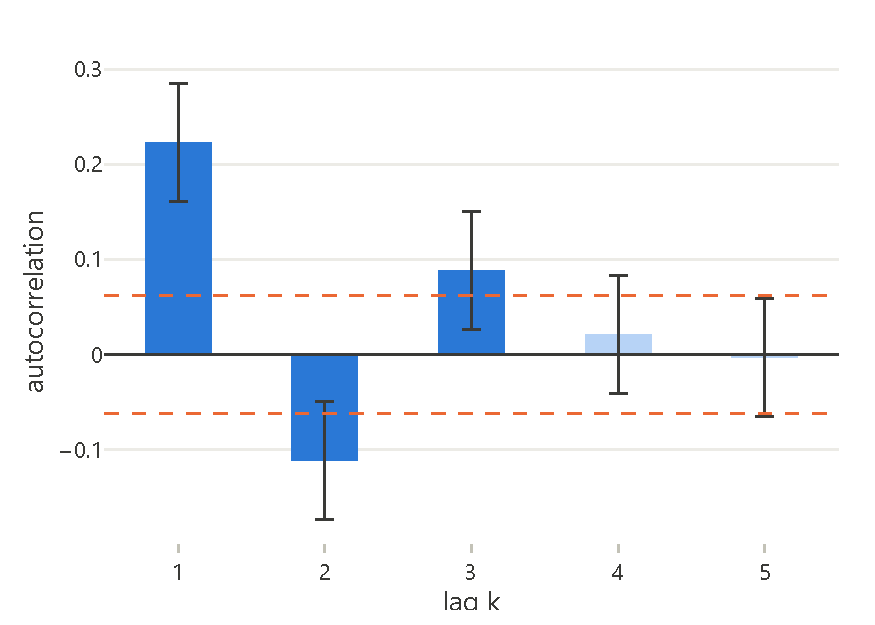
\includegraphics[width=\linewidth]{fig_acf_r}\end{minipage}\hfill
  \begin{minipage}{0.495\linewidth}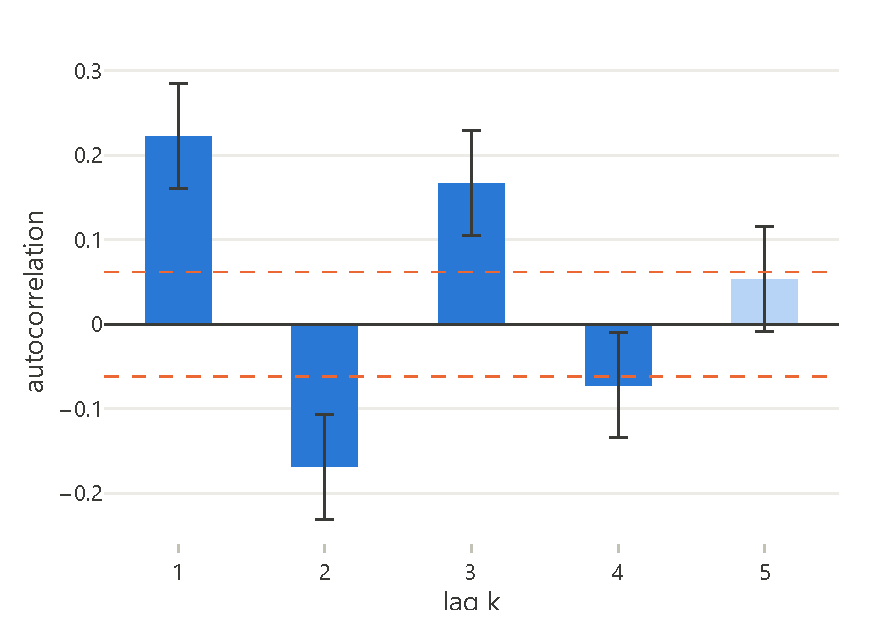
\includegraphics[width=\linewidth]{fig_pacf_r}\end{minipage}
  \caption{Correlogram (left) and PACF (right) of $r_t$. Whiskers: $\pm 1.96/\sqrt{T}$ around each estimate;
           dashed lines: $\pm\band$ around zero. Dark bars are significant at 5\%.}
  \label{fig:acf_r}
\end{figure}

\begin{figure}[ht]
  \centering
  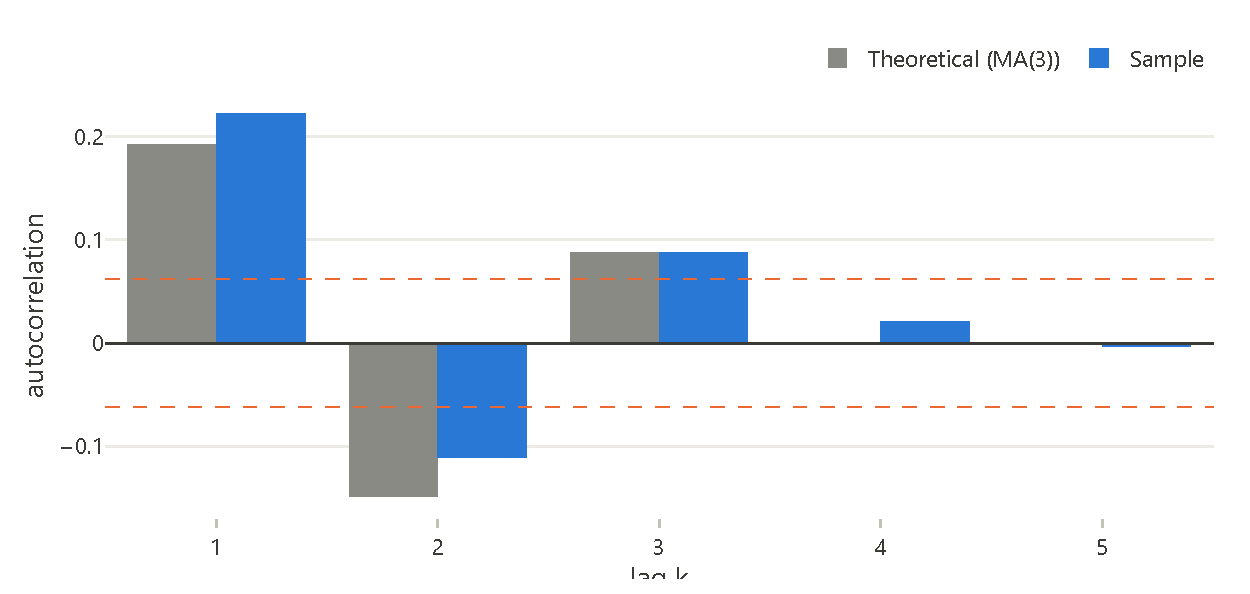
\includegraphics[width=0.8\linewidth]{fig_theory_r}
  \caption{Theoretical ACF of the MA(3) against the sample ACF of $r_t$.}
  \label{fig:theory_r}
\end{figure}

\begin{discussion}{Group discussion 1: Does our estimated process behave as expected?}
\todo{100--120 words. Conclusion first; cite specific lags and values from Table~\ref{tab:acf_r};
distinguish the theoretical properties of the MA(3) from what this sample shows.}
\end{discussion}

\subsection{Variance ratio (1e)}
\todo{1--2 sentences: $VR(5)=\VRr$, $z=\zVRr$; $H_0$ and conclusion (Table~\ref{tab:joint}).}

\begin{table}[ht]
  \centering
  \caption{Joint tests of serial dependence.
           Ljung--Box $H_0$: $\rho_1=\dots=\rho_5=0$.
           Variance ratio $H_0$: random walk, $VR(5)=1$.}
  \label{tab:joint}
  \small
  \begin{tabular}{lrr}
\toprule
 & $r_t$ & $u_t$ \\
\midrule
Ljung--Box $Q_5$ & 70.229 & 8.549 \\
\quad $p$ ($\chi^2_5$) & $<0.001$ & 0.128 \\
$VR(5)$ & 1.307 & 1.023 \\
$\mu_r(5) = VR(5)-1$ & 0.307 & 0.023 \\
\quad $z$ & 4.420 & 0.329 \\
\quad $p$ ($N(0,1)$) & $<0.001$ & 0.742 \\
\bottomrule
\end{tabular}

\end{table}

\begin{discussion}{Group discussion 2: Are our tests telling the same story?}
\todo{100--120 words. Interpret $VR(5)$ in words; compare individual ACF tests, Ljung--Box and VR at 5\%;
explain, using the signs of the autocorrelations, why the tests need not always agree.}
\end{discussion}

% ==================================================================
\section{Exercise 2: returns equal to $u_t$}
% ==================================================================

\subsection{Normality (2a)}
\todo{1--2 sentences on Table~\ref{tab:normality} for $u_t$ and on Figure~\ref{fig:dist_u}.}

\begin{figure}[ht]
  \centering
  \begin{minipage}{0.495\linewidth}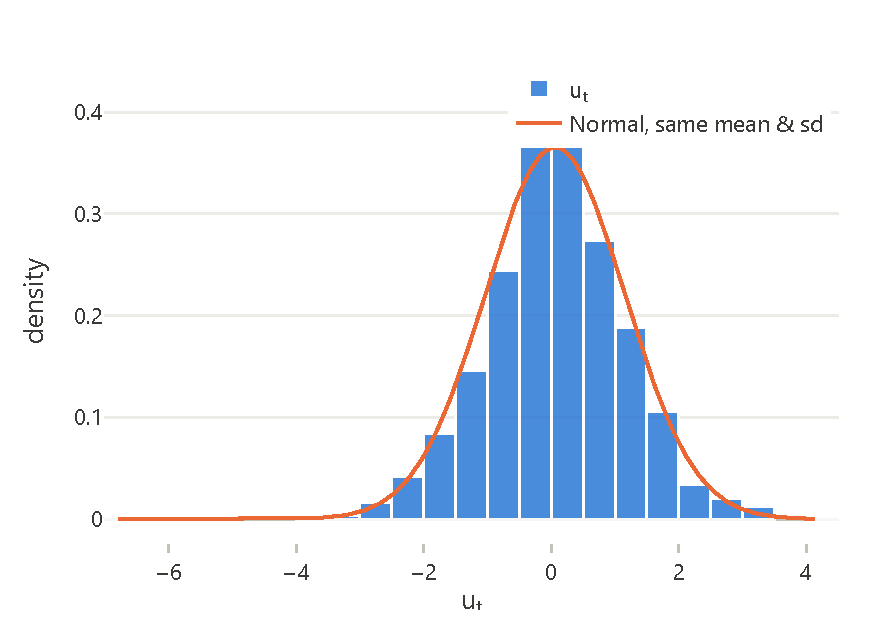
\includegraphics[width=\linewidth]{fig_hist_u}\end{minipage}\hfill
  \begin{minipage}{0.495\linewidth}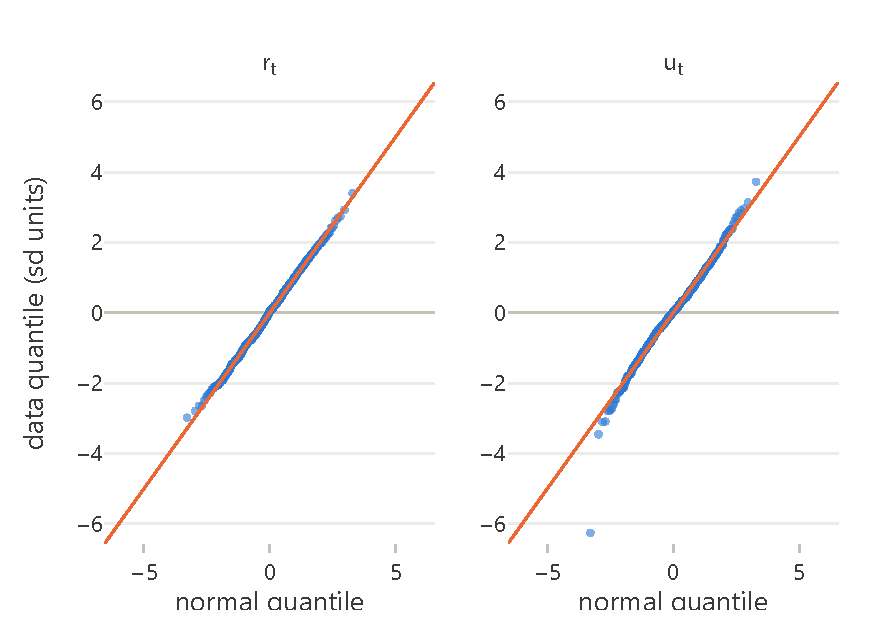
\includegraphics[width=\linewidth]{fig_qq}\end{minipage}
  \caption{Distribution of $u_t$: histogram with the normal density of equal mean and variance (left), and
           Q--Q plots of $r_t$ and $u_t$ against the normal (right).}
  \label{fig:dist_u}
\end{figure}

\subsection{Autocorrelations, partial autocorrelations and variance ratio (2b--2d)}
\todo{Short description of Table~\ref{tab:acf_u}, Figure~\ref{fig:acf_u} and the $u_t$ column of Table~\ref{tab:joint}
($Q_5=\Qu$, $VR(5)=\VRu$, $z=\zVRu$).}

\begin{table}[ht]
  \centering
  \caption{$u_t$: sample ACF (2b) and PACF (2c), $T=\Tu$. Tests as in Table~\ref{tab:acf_r}.}
  \label{tab:acf_u}
  \small
  \begin{tabular}{lrrrrrr}
\toprule
Lag $k$ & $\hat\rho_k$ & $z$ & $p$ & $\hat\phi_{kk}$ & $z$  & $p$  \\
\midrule
1 & 0.047 & 1.491 & 0.136 & 0.047 & 1.491 & 0.136 \\
2 & -0.049 & -1.549 & 0.121 & -0.051 & -1.623 & 0.105 \\
3 & 0.012 & 0.389 & 0.697 & 0.017 & 0.544 & 0.586 \\
4 & -0.028 & -0.880 & 0.379 & -0.032 & -1.011 & 0.312 \\
5 & -0.054 & -1.720 & 0.085 & -0.050 & -1.587 & 0.113 \\
\bottomrule
\end{tabular}

\end{table}

\begin{figure}[ht]
  \centering
  \begin{minipage}{0.495\linewidth}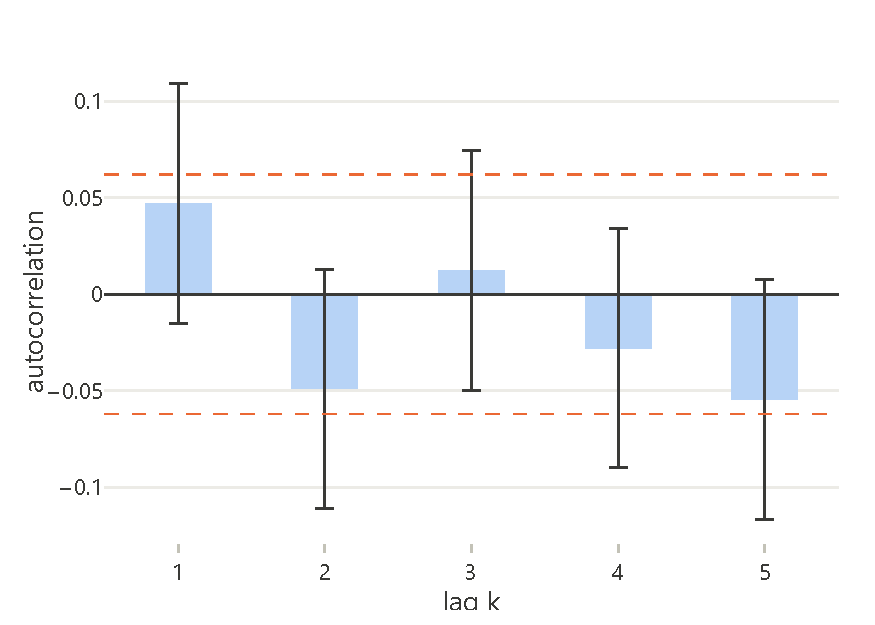
\includegraphics[width=\linewidth]{fig_acf_u}\end{minipage}\hfill
  \begin{minipage}{0.495\linewidth}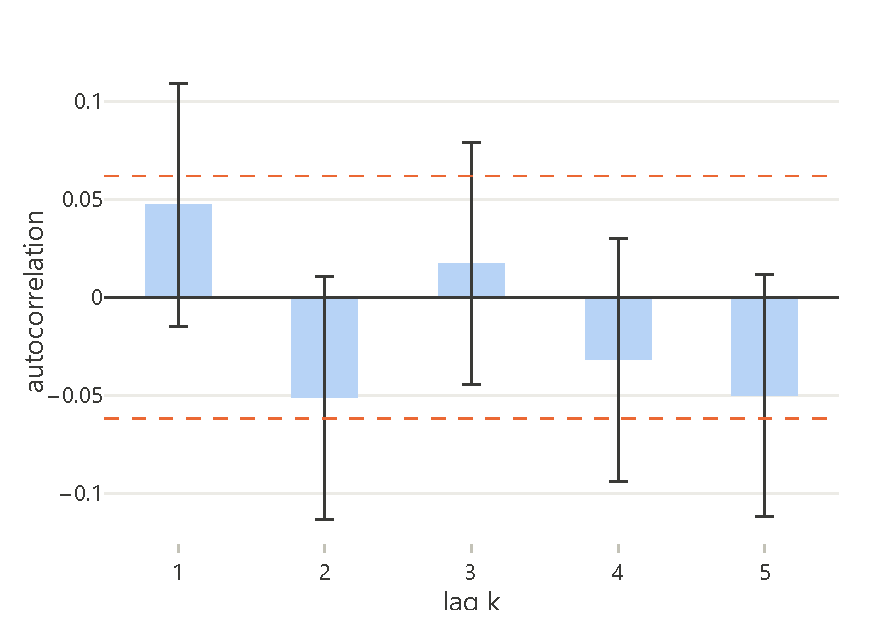
\includegraphics[width=\linewidth]{fig_pacf_u}\end{minipage}
  \caption{Correlogram (left) and PACF (right) of $u_t$. Bands as in Figure~\ref{fig:acf_r}.}
  \label{fig:acf_u}
\end{figure}

\begin{discussion}{Group discussion 3: What have we learned about the two return series?}
\todo{100--120 words. Compare $r_t$ and $u_t$ on distributional shape and on serial dependence, citing
Tables~\ref{tab:normality}--\ref{tab:joint}; say which results would survive reordering $u_t$;
state the strongest conclusion about linear dependence and one limitation.}
\end{discussion}

% ==================================================================
\section*{Record of group discussion}
% ==================================================================
\todo{At most 60 words: an interpretation the group challenged, the evidence considered,
and why the conclusion was revised or retained. Agreement from the outset is acceptable.}

% ==================================================================
\section*{Use of AI}
% ==================================================================
\todo{State briefly what AI helped with and how you checked it.}

\end{document}
